\subsection{09.11.18}
\subsubsection{Вероятностное пространство}
Пусть S - конечное множество, $|S| = n$.\\
Пусть задана функция $f: S \rightarrow [0, 1]$, $\forall \omega \in S \exists ! f(\omega) \in [0, 1]$.\\
$\sum\limits_{\omega \in S} f(\omega) = 1$\\
Определим $\forall A \subseteq S \; Pr(A) = \sum\limits_{\omega \in A} f(\omega)$, в частности:\\
$Pr(\varnothing) = 0$\\
$Pr(S) = 1$\\
$Pr(\{\omega\}) = f(\omega)$\\
В этот момент получается, что исходная функция f нам как бы уже не нужна, нам достаточно иметь Pr.\\
$(S, Pr)$ собственно и называется вероятностным пространством.\\
S называют пространством элементарных событий,\\
$\omega \in S$ - элементарным событием (исходом),\\
$A \subseteq S$ - событием\\
Pr(A) - вероятностью A\\
$A, B \subseteq S, Pr(A \cap B) = 0$ - несовместными событиями.\\
$Pr\{P(x)\}$ - таким образом мы будем обозначать вероятность $P(\{\omega \in S \; : \; P(\omega)\})$ множества таких элементарных исходов в S, что для них выполняется условие P. Причем условие мы можем записывать в вольном формате, например $Pr\{$Сборная России по футболу выиграет чемпионат мира$\}$.
\subsubsection{Свойства вероятности}
\begin{itemize}
\item $\forall A, B \subseteq S \; Pr(A \cup B) = Pr(A) + Pr(B) - Pr(A \cap B)$ (формула включений и исключений). Доказательство: $Pr(A \cup B) = \sum\limits_{\omega \in A \cup B} f(\omega) = \sum\limits_{\omega \in A} f(\omega) + \sum\limits_{\omega \in B} f(\omega) - \sum\limits_{\omega \in A \cap B} f(\omega)$\\
\item $\forall A \subseteq S \; \overline{A} = S \setminus A$. $Pr(A) + Pr(\overline{A}) = 1$. Доказывается из определения вероятности. \\
\item $Pr(A \cup B) \leq Pr(A) + Pr(B)$. Очевидно из пункта 1 и того факта, что вероятность неотрицательна.\\
\item $Pr(A) = Pr(A \ B) + Pr(A \cap B)$
\end{itemize}
\subsubsection{Парадокс Монти Холла}
Ааааааавтомобииииль! (С)\\
На некотором телешоу ведущий предлагает игроку выбрать одну из трех дверей. Известно, что за одной из дверей находится автомобиль, а за двумя другими - по козе. После того как игрок сделал выбор, ведущий открывает одну из двух оставшихся дверей (причем обязательно ту, за которой коза, открыть дверь с автомобилем он не может) и предлагает игроку изменить выбор. Вопрос, собственно, в том, стоит ли менять выбор?\\
Для начала формализуем задачу:\\
\begin{itemize}
\item Нет оснований полагать, что приз скорее за одной дверью, чем за другой (организаторы выбирали дверь наугад)\\
\item Нет оснований полагать, что игрок предпочитает одну дверь другой (игрок выбирает дверь наугад)\\
\item Нет оснований полагать, что если у ведущего есть выбор, он предпочтет одну дверь другой\\
\item Нет оснований полагать, что кто-то из участников процесса нарушает правила игры\\0
\end{itemize}
Исходя из этого, построим дерево вариантов:\\
\begin{figure}
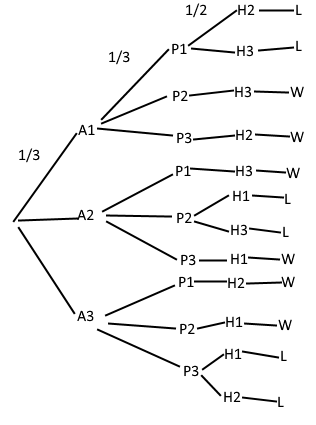
\includegraphics[width=\linewidth]{MontyHall.png}
\caption{Дерево вариантов}
\label{fig:MontyHall}
\end{figure}
Итак, сначала организаторы случайно (то есть, вероятность каждого из трех выборов - $\frac{1}{3}$) выбирают дверь, за которой помещают автомобиль (A1, A2, A3). Затем игрок делает свой выбор (P1, P2, P3), тоже случайно. Затем ведущий выбирает, какую дверь ему открыть. Заметим, что выбор у ведущего есть только если игрок исходно выбрал дверь, за которой находится приз. В таком случае, мы считаем, что ведущий делает выбор случайным образом (то есть, вероятность каждого из 2 выборов - $\frac{1}{2}$). Таким образом, мы получили набор элементарных исходов (листья дерева), каждый из которых имеет вид (Ax, Py, Hz) - выбор организаторов, выбор игрока, выбор ведущего. Вероятность каждого из таких исходов можно посчитать как произведение вероятностей на пути из корня дерева в лист, соответствующий данному исходу (то есть, $Pr(\{(A1, P1, H2)\}) = \frac{1}{3} * \frac{1}{3} * \frac{1}{2} = \frac{1}{18}$). Теперь нам нужно посчитать $Pr\{$Игрок выиграет, если сменит выбор$\}$. На картинке все исходы, удовлетворяющие этому условию, отмечены буквой W. Посчитав сумму их вероятностей, получим $\frac{2}{3}$.\\
Почему так получается? Очень грубо и не совсем корректно, зато интуитивно понятно, это можно объяснить так: вероятность того, что игрок исходно угадал - $\frac{1}{3}$. То есть с вероятностью $\frac{2}{3}$ автомобиль за одной из двух других дверей. Когда ведущий открывает дверь, мы не получаем никакой новой информации, т.к. заранее известно, что он должен был открыть дверь с козой. Значит, исходные $\frac{2}{3}$ вероятности, что игрок выбрал не ту дверь, остаются и сосредотачиваются на оставшейся двери, а значит, сменив выбор, игрок с вероятностью $\frac{2}{3}$ выиграет.\\
Еще до кучи всяких примеров с бросками монетки, бросками кубиков, вытягиванием карт, игрой в русскую рулетку и.т.д можно придумать и самим.
\subsubsection{Условная вероятность}
Пусть есть вероятностное пространство $(S, PR)$, $A, B \subseteq S$, $Pr(B) \not= 0$. Тогда вероятностью A при условии B (вероятность события A при условии, что известно, что событие B произошло) называют \\
$Pr(A|B) = \frac{Pr(A \cap B)}{Pr{B})}$.\\
\subsubsection{Задача о хоккейной команде}
ХК Локомотив играет серию до двух побед против СКА. Вероятность того, что Локомотив выиграет первую игру - $\frac{1}{2}$, а вот для остальных игр действует правило: если Локомотив выиграл предыдущую игру, вероятность его победы поднимается до $\frac{2}{3}$, а если проиграл - падает до $\frac{1}{4}$. Построим дерево возможных вариантов:\\
\begin{figure}
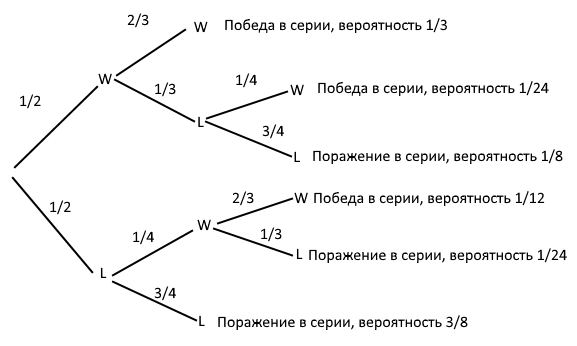
\includegraphics[width=\linewidth]{Hockey.png}
\caption{Дерево вариантов}
\label{fig:Hockey}
\end{figure}
Построим множество элементарных исходов $S = \{WW, WLW, WLL, LWW, LWL, LL\}$\\
Посчитаем несколько вероятностей:\\
\begin{itemize}
\item $Pr\{$Локомотив выиграет серию$\} = Pr(\{WW, WLW, LWW\}) = \frac{1}{3} + \frac{1}{24} + \frac{1}{12} = \frac{11}{24}$\\
\item $Pr\{$Локомотив выиграет серию, если он выиграл первую игру$\} = Pr(\{WW, WLW, LWW\}|\{WW, WLW, WLL\}) = \frac{Pr(\{WW, WLW\})}{Pr(\{WW, WLW, WLL\})} = \frac{\frac{1}{3} + \frac{1}{24}}{\frac{1}{2}} = \frac{3}{4}$\\
\item $Pr\{$Локомотив выиграл первую игру, если он выиграл серию$\} = Pr(\{WW, WLW, WLL\}|\{WW, WLW, LWW\}) = \frac{Pr(\{WW, WLW\})}{Pr(\{WW, WLW, LWW\})} = \frac{\frac{1}{3} + \frac{1}{24}}{\frac{1}{2}} = \frac{9}{11}$\\
\item $Pr\{$Локомотив выиграет вторую игру, если он выиграл первую игру$\} = Pr(\{WW, LWW, LWW\}|\{WW, WLW, WLL\}) = \frac{Pr(\{WW\})}{Pr(\{WW, WLW, WLL\})} = \frac{\frac{1}{3}}{\frac{1}{2}} = \frac{2}{3}$
\end{itemize}